\begin{figure}[hbtp]
  \centering
  \subfigure{
    \label{fig:rak-pruning--all}
    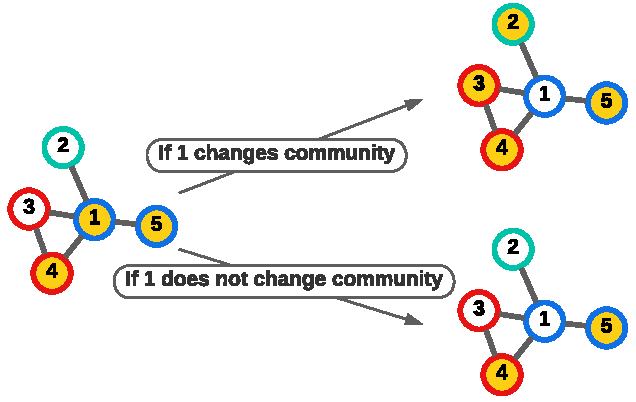
\includegraphics[width=0.78\linewidth]{out/rak-pruning.pdf}
  } \\[-2ex]
  \caption{Illustration of vertex pruning optimization: Once vertex $1$ is processed, it is unmarked. If vertex $1$ changes its community, its neighbors are marked for processing. Community membership of each vertex is indicated by border color, and marked vertices are highlighted in yellow \cite{sahu2023gvelouvain}.}
  \label{fig:rak-pruning}
\end{figure}
